% !TEX root = ../thesis-sample.tex

\chapter{LSPR response to Bovine Serum Albumin} \label{chap:lspr_response_bsa}
\graphicspath{{lspr_response_bsa/figs/}}

Localized surface plasmon resonance (LSPR) biosensors detect target molecules
by tracking frequency shifts in the plasmon resonance of metallic nanoparticles
in the presence of analytes \cite{WilletsVandyune2007}. The chapter presents the 
modeling of LSPR biosensors using \pygbe. We compute the extinction cross section 
of a silver nanosphere with bovine serum albumin (BSA) proteins (PDB code: 4FS5,
BSA dimmer) in different locations around it. 


{\color{red}
We might need to add something else here
}

\section{Grid convergence analysis} \label{sec:grid_conv_bsa}
We perform a grid convergence study to ensure that the meshes are correctly
resolving the numerical solutions. We performed the convergence analysis of
the system sketched in in Figure \ref{fig:analyte-sensor}. Given that we 
compute the extinction cross section by integrating over the sphere, we set 
a fixed mesh density for the protein and refined the mesh of the nanosphere 
(512, 2048, 8192, 32768 elements). For the protein, we found that a mesh with
two triangles per $\text{\AA}^2$ was fine enough for the convergence 
analysis, resulting in $N_{prot} = 98116$ elements.
We use the same conditions used in the grid convergence analysis of the 
isolated nanoparticle of section \ref{sub_sec:grid_conv_iso}, presented
in Tables \ref{table:quadparams1} and \ref{table:treeparams1}. The protein 
dielectric constant for a wavelngth of 380 nm is $2.7514 + 0.2860i$, this  
value was computed using a functional relationship provided by Phan
 et al.~\cite{PhanETal2013}. The protein was located at a distance of 
 $d=$ 1 nm of the sphere along the z-axis, such that its dipole moment 
 was aligned with the y-axis. We show the errors in Figure  \ref{fig:err_sph-bsa} 
 and table \ref{table:err_sph-bsa} which were computed using the Richardson extrapolated
{\color{red} (see Section, cite section that explains rich extra)} value of 
the extinction cross section $C_{ext}= 1778.73$ nm$^2$.

\begin{figure}%[h] %  figure placement: here, top, bottom, or page
    \centering
    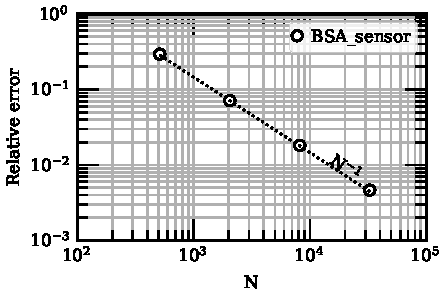
\includegraphics[width=0.65\textwidth]{convergence_bsa_sensor_R8_d1_w380.pdf} 
    \caption{Grid-convergence study of extinction cross-section of a spherical silver
             nanoparticle with a BSA protein at $d=1$ nm. 
             Figure, plotting script and auxiliary files available 
             under \textsc{cc-by} \cite{ClementiETal2018c}.}
    \label{fig:err_sph-bsa}
 \end{figure}

 \begin{table}%[h]
    \centering
    \caption{\label{table:err_sph-bsa} Estimated percentage error of the BSA-sensor 
    system (Fig.~\ref{fig:analyte-sensor}), with respect to the extrapolated value 
    (using Richardson extrapolation).} 
    \begin{tabular}{c c}
    \hline%\toprule
    N & \% error \\
    \hline%\midrule
     $512$ & $29.39$ \\
     $2048$ & $7.13$ \\
     $8192$ & $1.82$ \\
     $32768$ & $0.46$ \\
    \hline%\bottomrule
    \end{tabular}
\end{table}

The observed order of convergence is 0.99, and we can see in Figure
 \ref{fig:err_sph-bsa} that the error decays with the number of boundary elements
 at a rate of $1/N$, which is consistent with the verifications results showed
 in Section \ref{sec:verification}. This shows that the numerical solutions computed
 with \pygbe are correctly resolved by the meshes.

\section{Plasmon resonance frequency shifts} \label{sec:shift_bsa}

\section{Sensitivity study} \label{sec:sensitivity}
